\section{Introduction}

Road vehicles require a network of roads and a network of \glspl{ras} whose nodes are coincident with a subset of the nodes of the road network. Allocation of \glspl{ras} to road network nodes is a central concern in transportation planning. To a great extent, the topology of the \gls{ras} network will be determined by the topology of the road network, itself determined by and determinative of population and economic topology. In other words, roads connect places, \glspl{ras} serve vehicles on roads. It is unlikely that, for the sake of the \gls{ras} network, new roads will be built or population concentrations will shift. Thus, the problem of optimal resource allocation, with respect to \glspl{ras} should aim to propose locations for \glspl{ras} such that the performance of the road network is maximized with respect to the demand generated by population and economic topology.

When designing a system, the initial stages of the design should make explicit the relative importance of objectives in conflict. A common conflict is efficiency vs. resilience. There are many definitions of resilience but, in general, systems which ar more redundant are more resilient. It is intuitive to view efficiency and redundancy as conflicting objectives. From the point of view of a \gls{ras} network, the most efficient system is one wherein every \gls{ras} is at full capacity at all times. For such a network, user delays due to queuing are guaranteed. Although more efficient and, thus, able to charge less per unit energy delivered, consumers will find the experience annoying and the market will correct providing some redundancy. From the perspective of the road network, significant \gls{ras} redundancy may be called for in certain areas where individual stations are very inefficient. In order to make the road network functional, inefficient \glspl{ras} must be funded via incentives, the effectiveness of which will depend on how well station locations are optimized.

%The redundancy of a system, or even how to measure redundancy, is not always apparent. It is common practice for the front and rear brakes on a car to be operated by independent hydraulic systems in order to maximize the likelihood of at least one axle's brakes working. This is a fairly clear case of redundancy being purchased at the cost of a few extra parts and slightly more difficult maintenance. However, the two hydraulic systems are joined at the brake pedal, if they were each further bifurcated then they would be joined at the caliper pistons as well. Doubling the number of independent hydraulic systems would not meaningfully increase redundancy.

Consider the scenario shown in Figure \ref{fig:connected_cities_1}. Cities 1 and 2 are connected by a single road with one \gls{ras} ($A$) located halfway between the cities. A vehicle with unlimited range could make the trip between the cities without stopping at $A$ but the maximum range of the relevant vehicle is greater than the distance from either city to $A$ but less than the distance between the cities.

\begin{figure}[H]
	\centering
	
\includegraphics[width = .66\linewidth]{figs/connected_cities_1.png}
	\caption{Cities connected by one road with one \gls{ras}. Solid lines indicate a link is sufficient to lead to a range addition event after traversal, dashed lines indicate the opposite, and dotted lines indicate a link which originates and/or terminates in a city.}
	\label{fig:connected_cities_1}
\end{figure}

Drivers heading from city 1 to city 2 and vice versa will have to utilize $A$. There are two consequences to this reliance: (1) should $A$ go offline then no traffic can make it from city 1 to city 2 and (2) since all traffic must utilize $A$ all vehicles will have to add range at equivalent stages of their trip. The second consequence is of greater importance if traffic between the cities is concentrated at certain time slots. Consider now a second set of cities, Cities 3 and 4 as in Figure \ref{fig:connected_cities_2} which are also connected by just one road but this road hosts three \glspl{ras} ($B$, $C$, and $D$).

\begin{figure}[H]
	\centering
	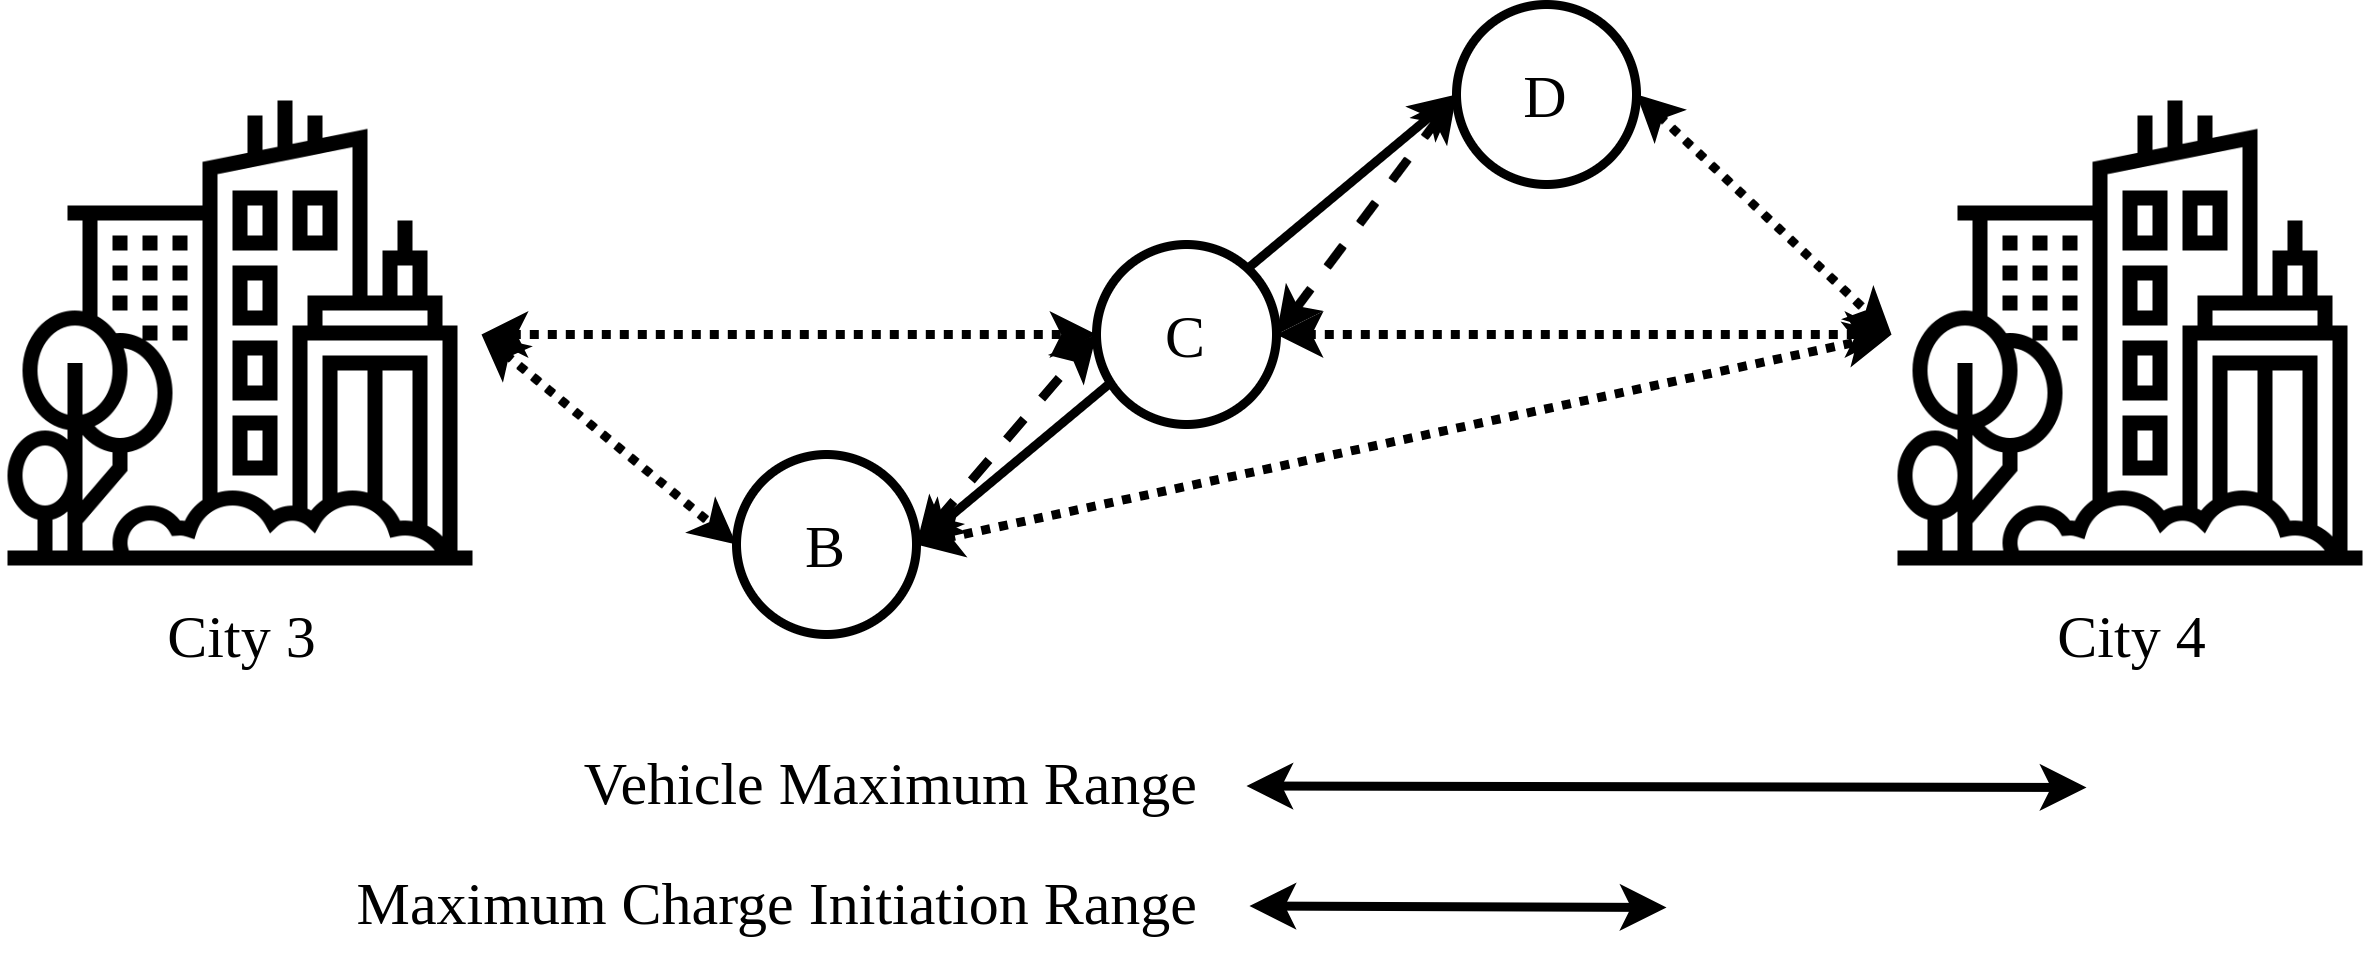
\includegraphics[width = .66\linewidth]{figs/connected_cities_2.png}
	\caption{Cities connected by one road with multiple \glspl{ras}. Solid lines indicate a link is sufficient to lead to a range addition event after traversal, dashed lines indicate the opposite, and dotted lines indicate a link which originates and/or terminates in a city.}
	\label{fig:connected_cities_2}
\end{figure}

Limited range vehicles have several options of, nominally, equal cost in this scenario. Consider the graph topology; $B$, $C$, and $D$ are reachable from City 4, $B$ and $C$ are reachable from City 3, and the \glspl{ras} are mutually within range. The 3 - 4 direction has two equivalent paths (3 - $B$ - 4 and 3 - $C$ - 4) and one higher cost path (3 - $B$ - $D$ -4). The 4 - 3 direction has three equivalent paths (through each station) and one higher cost path (4 - $D$ - $B$ - 3). In the first scenario there were only two shortest paths for travelers in cities 1 and 2, a number which increases to five for cities 3 and 4 with two additional viable paths. One might expect that, over time, drivers will tend to distribute themselves among the various paths thus reducing the expected wait time and the reliance on any one station. It should be noted, however, that the redundancy was not increased by adding stations but, rather, by adding stations in the locations in which they were added. If most cars begin their trips at roughly the same time then all will reach $C$ at roughly the same time but by the time cars from 3 reach $D$ most cars from 4 will be close to $B$. The optionality created by adding new stations as opposed to new chargers at the same station reduces demand coordination allowing expected queuing time to decrease without altering the vehicles per charger ratio. When traveling in the 3 - 4 direction one may observe that the choice boils down to "charge at $B$" or "charge at $C$". One is very unlikely to charge at $B$ and again at $C$ because the distance between the nodes and from $C$ to 4 is not great enough to justify it. Before node $B$ the driver had three viable paths, after passing node $B$ the driver has only one: much information is gained by passing node $B$.

Finally, consider the situation of cities 5 and 6 as seen in Figure \ref{fig:connected_cities_3}. Cities 5 and 6 are farther apart than the previous examples and are connected by two main roads.

\begin{figure}[H]
	\centering
	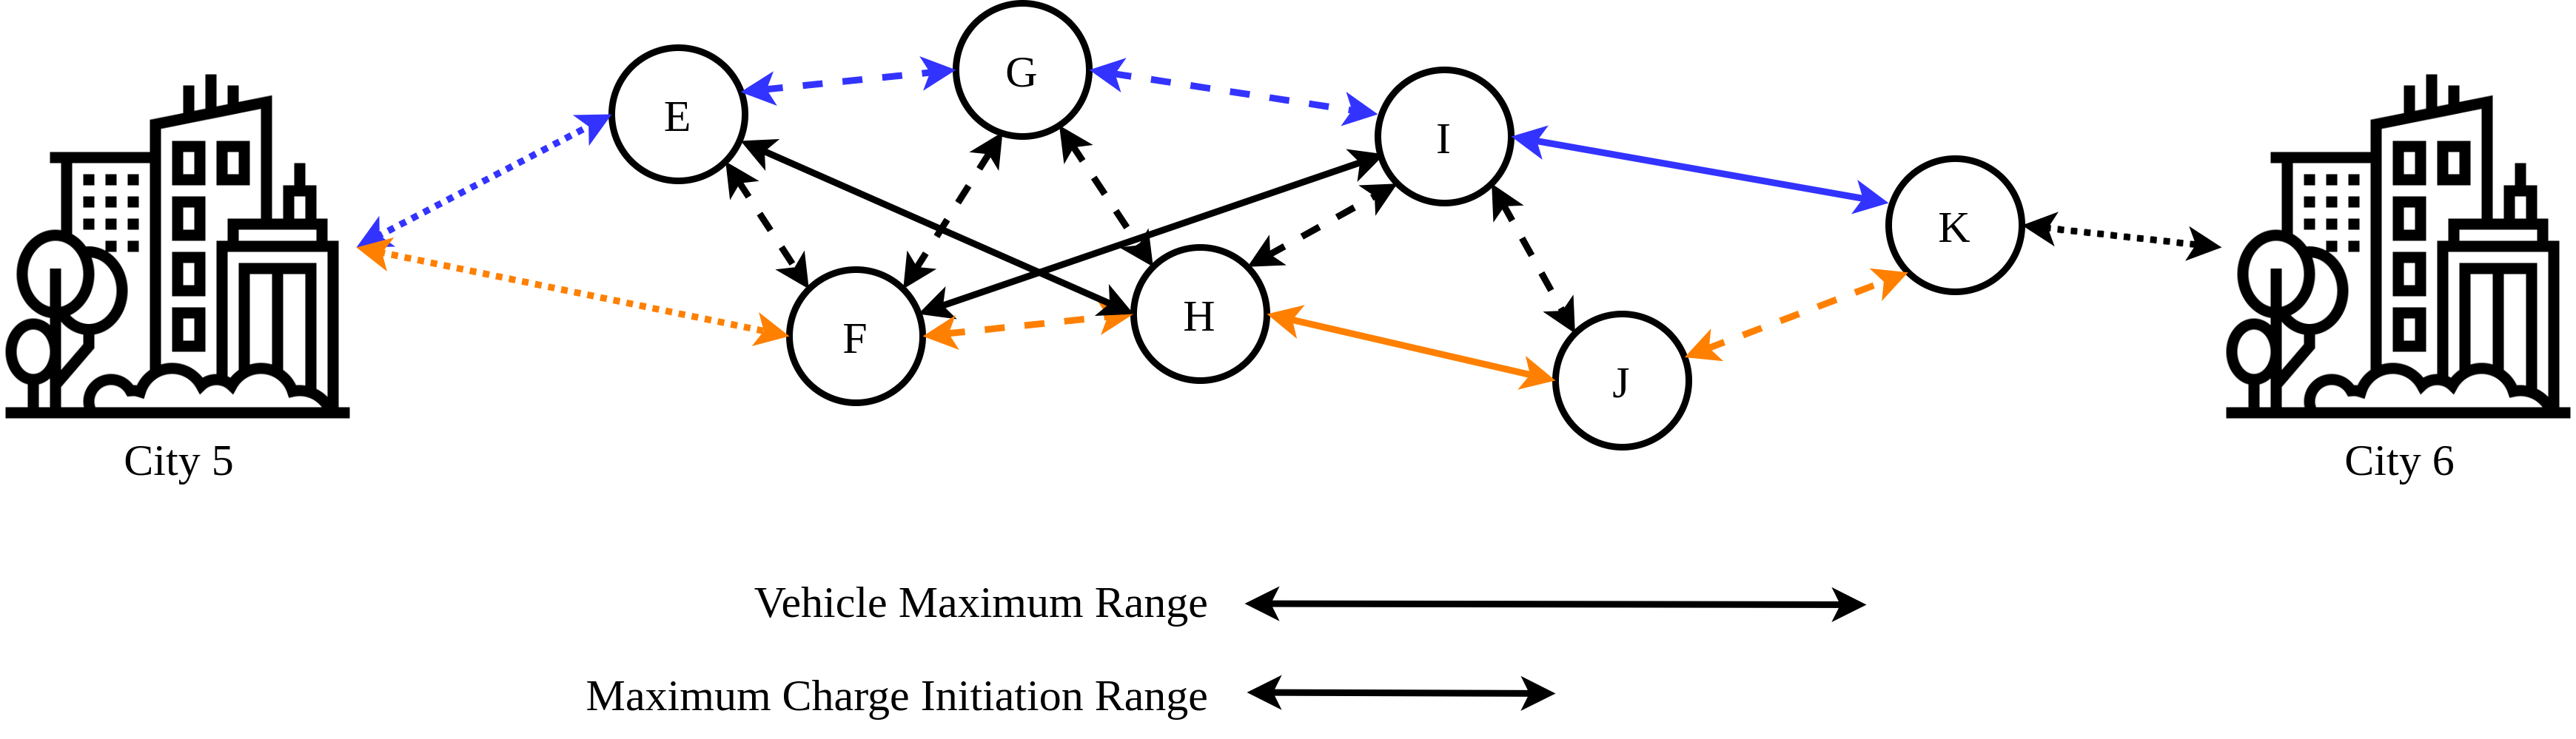
\includegraphics[width = \linewidth]{figs/connected_cities_3.png}
	\caption{Cities connected by multiple roads with multiple \glspl{ras}. Solid lines indicate a link is sufficient to lead to a range addition event after traversal, dashed lines indicate the opposite, and dotted lines indicate a link which originates and/or terminates in a city.}
	\label{fig:connected_cities_3}
\end{figure}

The upper main road (blue links) hosts stations $E$, $G$, $I$, and $K$ and the lower road (orange links) hosts stations $F$, $H$, and $J$. There are many secondary roads which connect the nodes of the main road and both main roads converge at $K$ before heading to city 6.